\documentclass[../../dissertation.tex]{subfiles}
\begin{document}
The staggered quantum walk (SQW) case aims to spread a transition probability to
neighboring vertices with discrete time steps. The notion of adjacency comes
from cliques\footnote{A clique is defined as the subset of vertices of an
	undirected graph such that every two distinct vertices in each clique
are adjacent.}, and the initial stage of this walk consists of partitioning the
graph in several different cliques. This is called tessellation, and it is
defined as the division of the set of vertices into disjoint cliques. An
element of a tessellation $\mathscr{T}$ is called a polygon, and it's only
valid if all of its vertices belong to the clique in $\mathscr{T}$. The set
of polygons of each tessellation must cover all vertices of the graph, and the
set of tessellations
($\mathscr{T}_{1}$,$\mathscr{T}_{2}$,...,$\mathscr{T}_{k}$) must cover all the
edges.\par 

These definitions allow the construction of operators $H_1$,$H_2$,...,$H_k$ to propagate the probability amplitude locally, in each
polygon. The state associated to each polygon is
\begin{equation}
	\ket{u_{j}^{k}} = \frac{1}{\sqrt{\mathopen|\alpha_{j}^{k}}\mathclose|}\sum_{l\in\alpha_{j}^{k}}\ket{l}
\end{equation}
where $\alpha_{j}^{k}$ is the $j^{th}$ polygon in the $k^{th}$ tessellation.\par

The unitary and Hermitian operator $H_k$, associated to each tessellation is
defined in \cite{portugal2017b} as
\begin{equation}
	H_k = 2\sum_{j=1}^{p}\ket{u_{j}^{k}}\bra{u_{j}^{k}} - I.
	\label{eq:StagHamil}
\end{equation}
Solving the time-independent Schrodinger equation for this Hamiltonian gives
the evolution operator 
\begin{equation}
	U = e^{i\theta_{k}H_{k}}...e^{i\theta_{2}H_{2}}e^{i\theta_{1}H_{1}}
	\label{eq:stagWalkUnmodOp}
\end{equation}
where
\begin{equation}
	e^{i\theta_{k}H_{k}} = \cos{(\theta_k)}I + i\sin{(\theta_k)}H_k
\end{equation}
since $H_k^2 = I$, meaning that the Hamiltonian is a projection operator that,
when expanded in a Taylor series, generates a local operator.\par

The simplest use case of this quantum walk model is the one-dimensional
lattice, where the minimum tessellations are
\begin{equation}
	\mathscr{T}_{\alpha}= \{\{2x,2x+1\}\colon x \in \mathbb{Z}\},
\end{equation}
\begin{equation}
	\mathscr{T}_{\beta}= \{\{2x+1,2x+2\}\colon x \in \mathbb{Z}\}.
\end{equation}
\begin{figure}[!h]
	\centering
	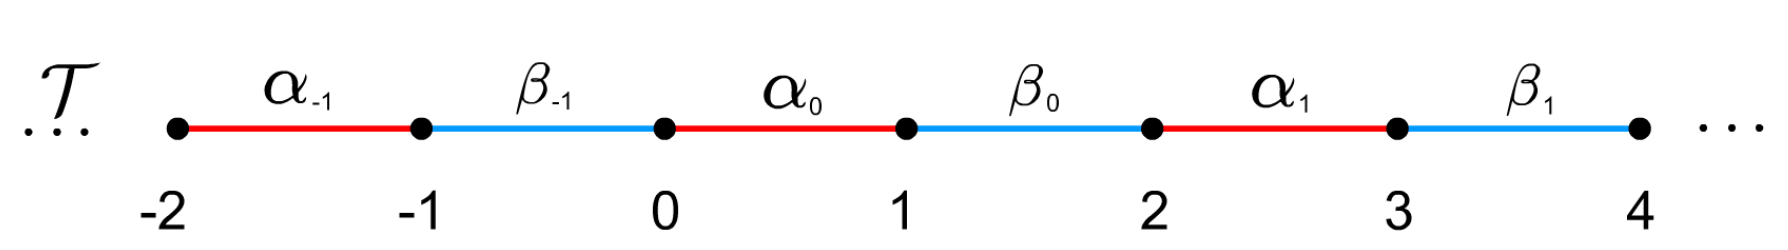
\includegraphics[scale=0.40]{img/StagQuantumWalk/tesselation.png}
	\caption{Tessellation of a line graph.} 
	\label{fig:stagQWTesselation}
\end{figure}
Each element of the tessellation has a corresponding state, as can be seen in
figure \ref{fig:stagQWTesselation}, and the uniform superposition of these
states is
\begin{equation}
	\ket{\alpha_x} = \frac{\ket{2x} + \ket{2x+1}}{\sqrt{2}}
\end{equation}
\begin{equation}
	\ket{\beta_x} = \frac{\ket{2x+1}+\ket{2x+2}}{\sqrt{2}}
\end{equation}
One can now define Hamiltonians $H_\alpha$ and $H_\beta$ as 
\begin{equation}
	H_\alpha = 2\sum_{x=-\infty}^{+\infty}\ket{\alpha_{x}}\bra{\alpha_x} - I
	\label{eq:stagSimulHalpha}
\end{equation}
\begin{equation}
	H_\beta = 2\sum_{x=-\infty}^{+\infty}\ket{\beta_{x}}\bra{\beta_x} - I
	\label{eq:stagSimulHbeta}
\end{equation}\par
The Hamiltonian evolution operator reduces to
\begin{equation}
	U = e^{i\theta H_\beta}e^{i\theta H_\alpha}
	\label{eq:stagSimulUniOp}
\end{equation}
and applying it to an initial condition $\ket{\psi(0)}$ results in the time
evolution operator
\begin{equation}
	U\ket{\psi(t)} = U^t\ket{\psi(0)}
\end{equation}\par
\begin{figure}[!h]
	\centering
	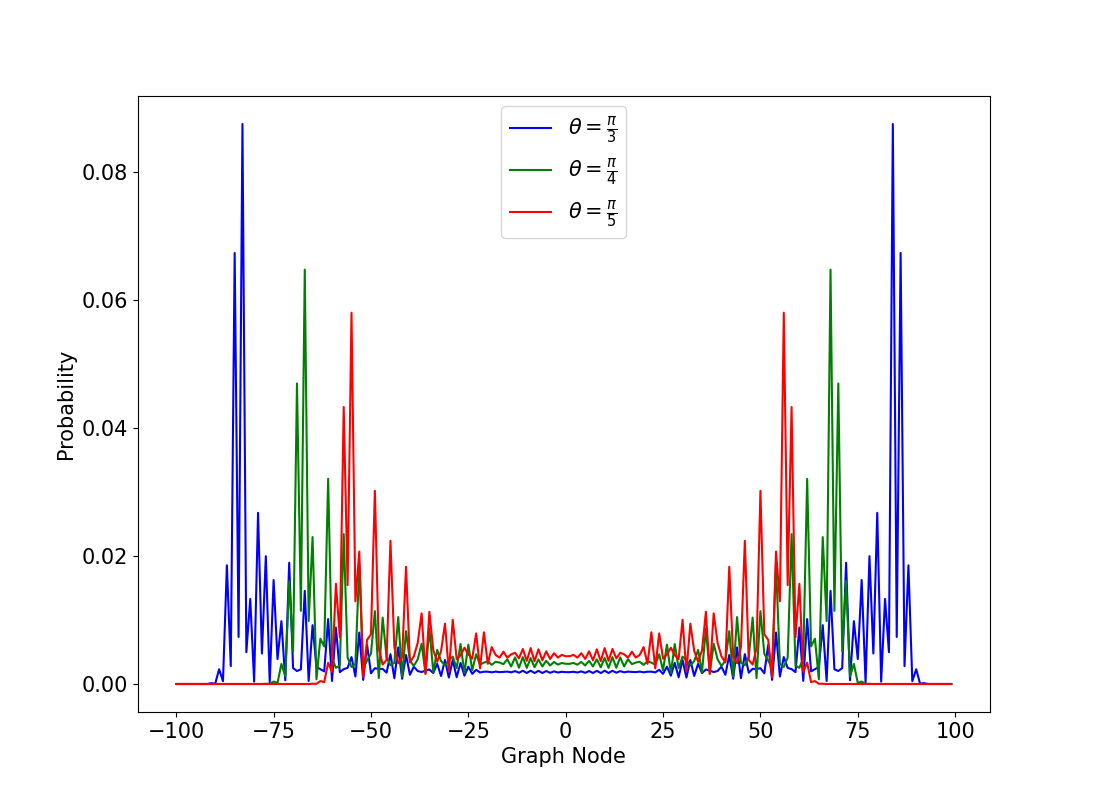
\includegraphics[scale=0.40]{img/StagQuantumWalk/stagqwMultiple.png}
	\caption{Probability distribution for the staggered quantum walk on a line after 50 steps, with initial condition $\ket{\psi(0)}=\frac{\ket{0}+\ket{1}}{\sqrt{2}}$, for multiple values of $\theta$.} 
	\label{fig:stagQWSimulMultTheta}
\end{figure}
Having defined the time evolution operator, the walk is ready to be coded with
a certain initial condition and $\theta$ value, to better understand how the
probability distribution spreads through time. 
%TODO:\textcolor{red}{você pode acrescentar que o $\theta$ terá um papel
%similar ao $\gamma$ no controle do desvio-padrão}
For the first case study, the initial condition will be a uniform superposition
of states $\ket{0}$ and $\ket{1}$ and the value of $\theta$ will be varied in
order to understand how this parameter impacts the walk, as can be seen in
figure \ref{fig:stagQWSimulMultTheta}. The overall structure of the
probability distribution is very similar for different values of $\theta$,
the difference being that the walker is more likely to be found further away
from the origin as the angle increases.\par

Another interesting case study is to see how the initial condition affects the
dynamics of the system, and figure \ref{fig:stagQW2InitCond} shows the results
of plotting the quantum walk for initial conditions  $\ket{\psi(0)}=\ket{0}$
and $\ket{\psi(0)}=\ket{1}$.
\begin{figure}[!h]
	\begin{subfigure}[h]{0.50\textwidth}
	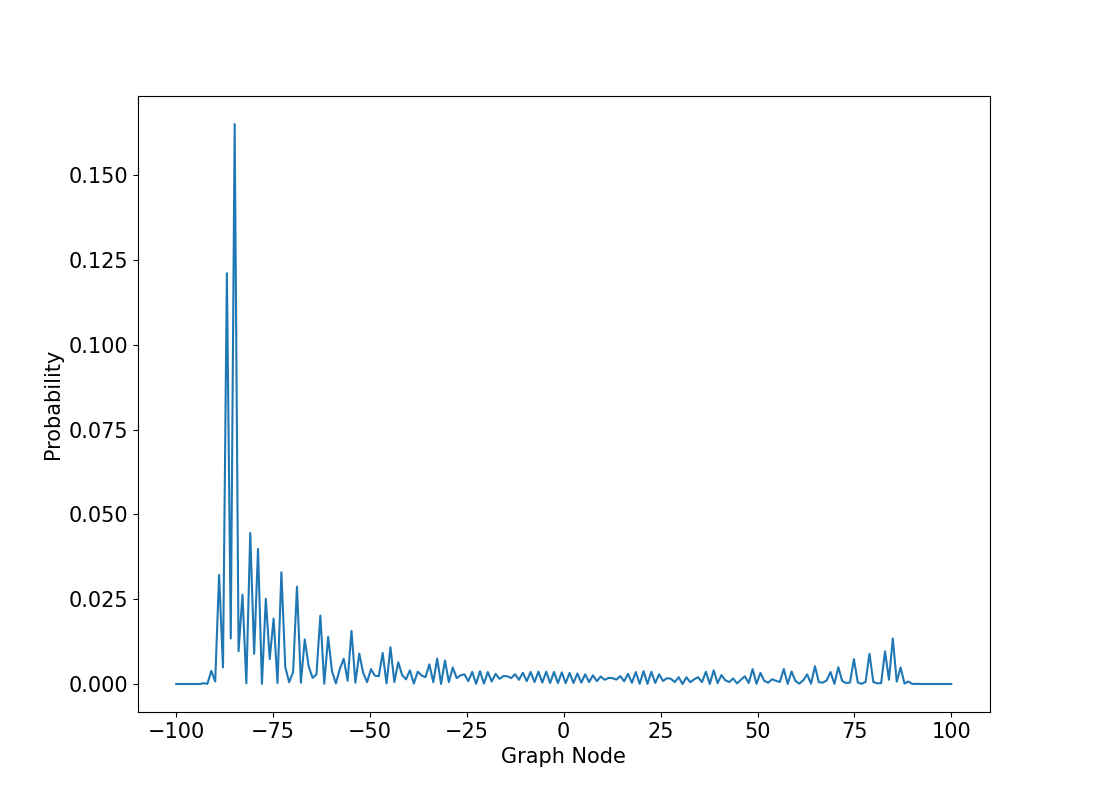
\includegraphics[width=\linewidth]{img/StagQuantumWalk/stagqwSingle0.png}
	\caption{$\ket{\psi(0)}=\ket{0}$}\label{fig:fig6}
	\end{subfigure}\hfill
	\begin{subfigure}[h]{0.50\textwidth}
	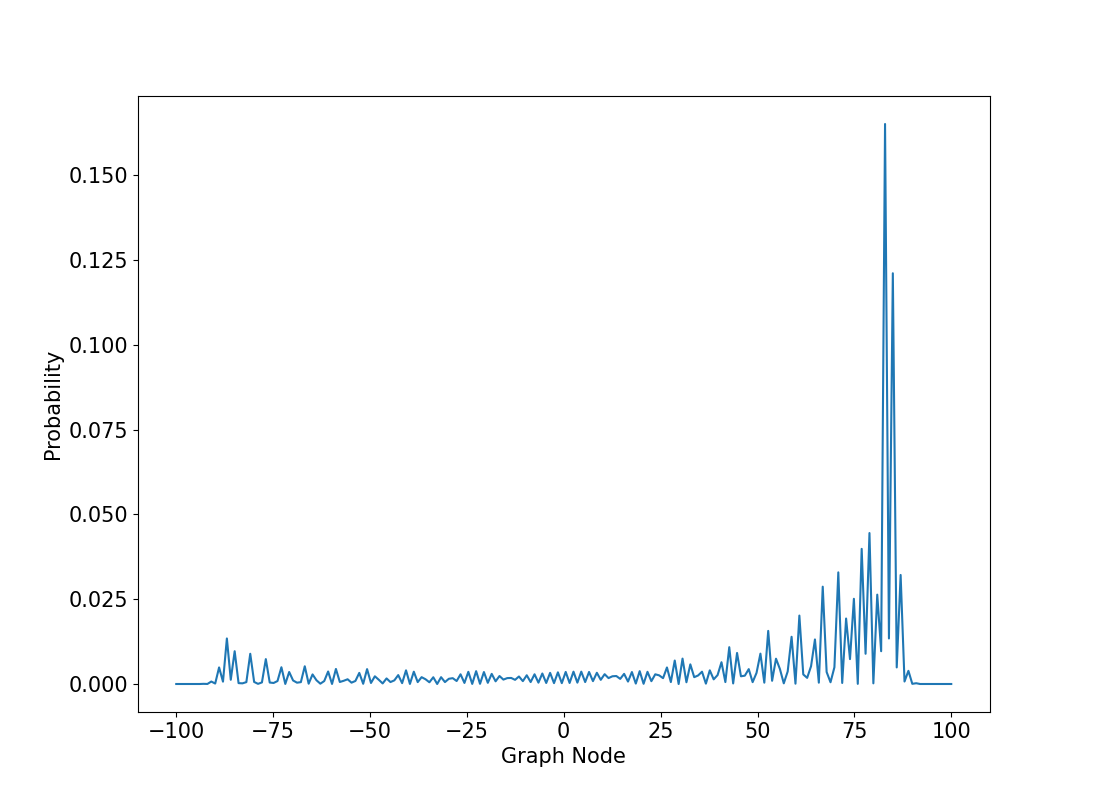
\includegraphics[width=\linewidth]{img/StagQuantumWalk/stagqwSingle1.png}
	\caption{$\ket{\psi(0)}=\ket{1}$}\label{fig:fig7}
	\end{subfigure}\hfill
	\caption{Probability distributions for the staggered quantum walk on a line after 50 steps, for different initial conditions.}
	\label{fig:stagQW2InitCond}
\end{figure}
Similarly to the coined case, each initial condition results in asymmetric
probability distributions, $\ket{\psi(0)}=\ket{0}$ leads to a peak  in the
left-hand side, while condition $\ket{\psi(0)}=\ket{1}$ results in a peak in the
right-hand side. As was shown in figure \ref{fig:stagQWSimulMultTheta}, the
uniform superposition of both these conditions results in a symmetric
probability distribution.\par So far, only discrete-time quantum walks have
been shown. The next section presents the continuous-time quantum walk model,
where time is not discretized and whose Hilbert space is proportional to the
space of the walker.

%TODO: \textcolor{red}{acho que você pode explicar um pouco mais o papel de $\theta$ através dos gráficos e podemos pensar se fazemos gráficos do desvio-padrão para este e o contínuo}


\end{document}
